\chapter{Literature Review }
%\Jnote{Capitalize ``review'' in the chapter title.}

In today's life, many organizations are generating unstructured data while they are communicating. There are plenty of entities to be extracted. In this research,  all reports we considered are written in English. 

To identify boundaries of sentences is one of the important prerequisite steps in Natural Language Processing. The punctuation marks cause some ambiguity  \citep{baluja2000applying} in texts processing.  For example, it is challenging to differentiate the point in abbreviations and a full stop. 

There are different approaches to extract entity from documents. Some information extractor (IE) systems are based on regular expressions rules and patterns between words. Other algorithms are based on machine learning concepts.

Named Entity Recognition  and Classification (NERC) is one or machine learning algorithms which uses  Markov Hidden Model to classify a document.

Due to various forms of contexts and forms various forms of documents, it is not preferable  to extract entities manually. Machine learning algorithms  give nice and robust results.

Parse tree is a graphical ordered representation of words compose sentences. It bases on rules of phase structure grammar. 


\section{ Parse  Tree} \label{tree}

One of the sentences that compose our sample report says: 
"Assessment reports indicated 117 deaths, 544 people injured, 12,794 homes damaged and 7,384 houses destroyed", Suppose that this sentence is called "S".

There are two mains steps which are performed to get the entities from   this sentence:
\begin{itemize}
\item \textbf{Tokenizing}: This is a procedure of taking a sentence and extracting the composing atomic linguistic elements i.e. words, verbs, punctuations, adjectives etc .
S has the following tokens: ['Assessment', 'reports', 'indicated', '117', 'deaths', ',', '544', 'people', 'injured', ',', '12,794', 'homes', 'damaged', 'and', '7,384', 'houses', 'destroyed']
\item \textbf{POS}: part-of-speech is a process of attaching to every linguistic element of the sentence a corresponding tag
based on grammar rules.
The POS of S  are: 
[('Assessment', 'JJ'), ('reports', 'NNS'), ('indicated', 'VBD'), ('117', 'CD'), ('deaths', 'NNS'), (',', ','), ('544', 'CD'), ('people', 'NNS'), ('injured', 'VBN'), (',', ','), ('12,794', 'CD'), ('homes', 'NNS'), ('damaged', 'VBN'), ('and', 'CC'), ('7,384', 'CD'), ('houses', 'NNS'), ('destroyed', 'VBD')]
\end{itemize}
The meanings of the used tags for S:
\begin{itemize}
\item JJ: \textbf{Adjective}: 'Assessment'.
\item NNS: \textbf{Noun, plural}: 'reports', 'deaths', 'people','houses'.
\item VBD: \textbf{Verbs, past tense}: 'indicated',             'injured', 'damaged', 'destroyed'.
\item CD: \textbf{Cardinal Number}: '117', '544' '12,794','7,384'.
\item CC: \textbf{Coordinate Conjugation}: 'and'
\end{itemize}
The parse tree is formed based on the POS. Classification and arrangement of words in a sentence determine the relationship between words. 
\begin{figure}[hbtp]
\caption{General Extraction Process \citep{bird2009natural} }
\centering
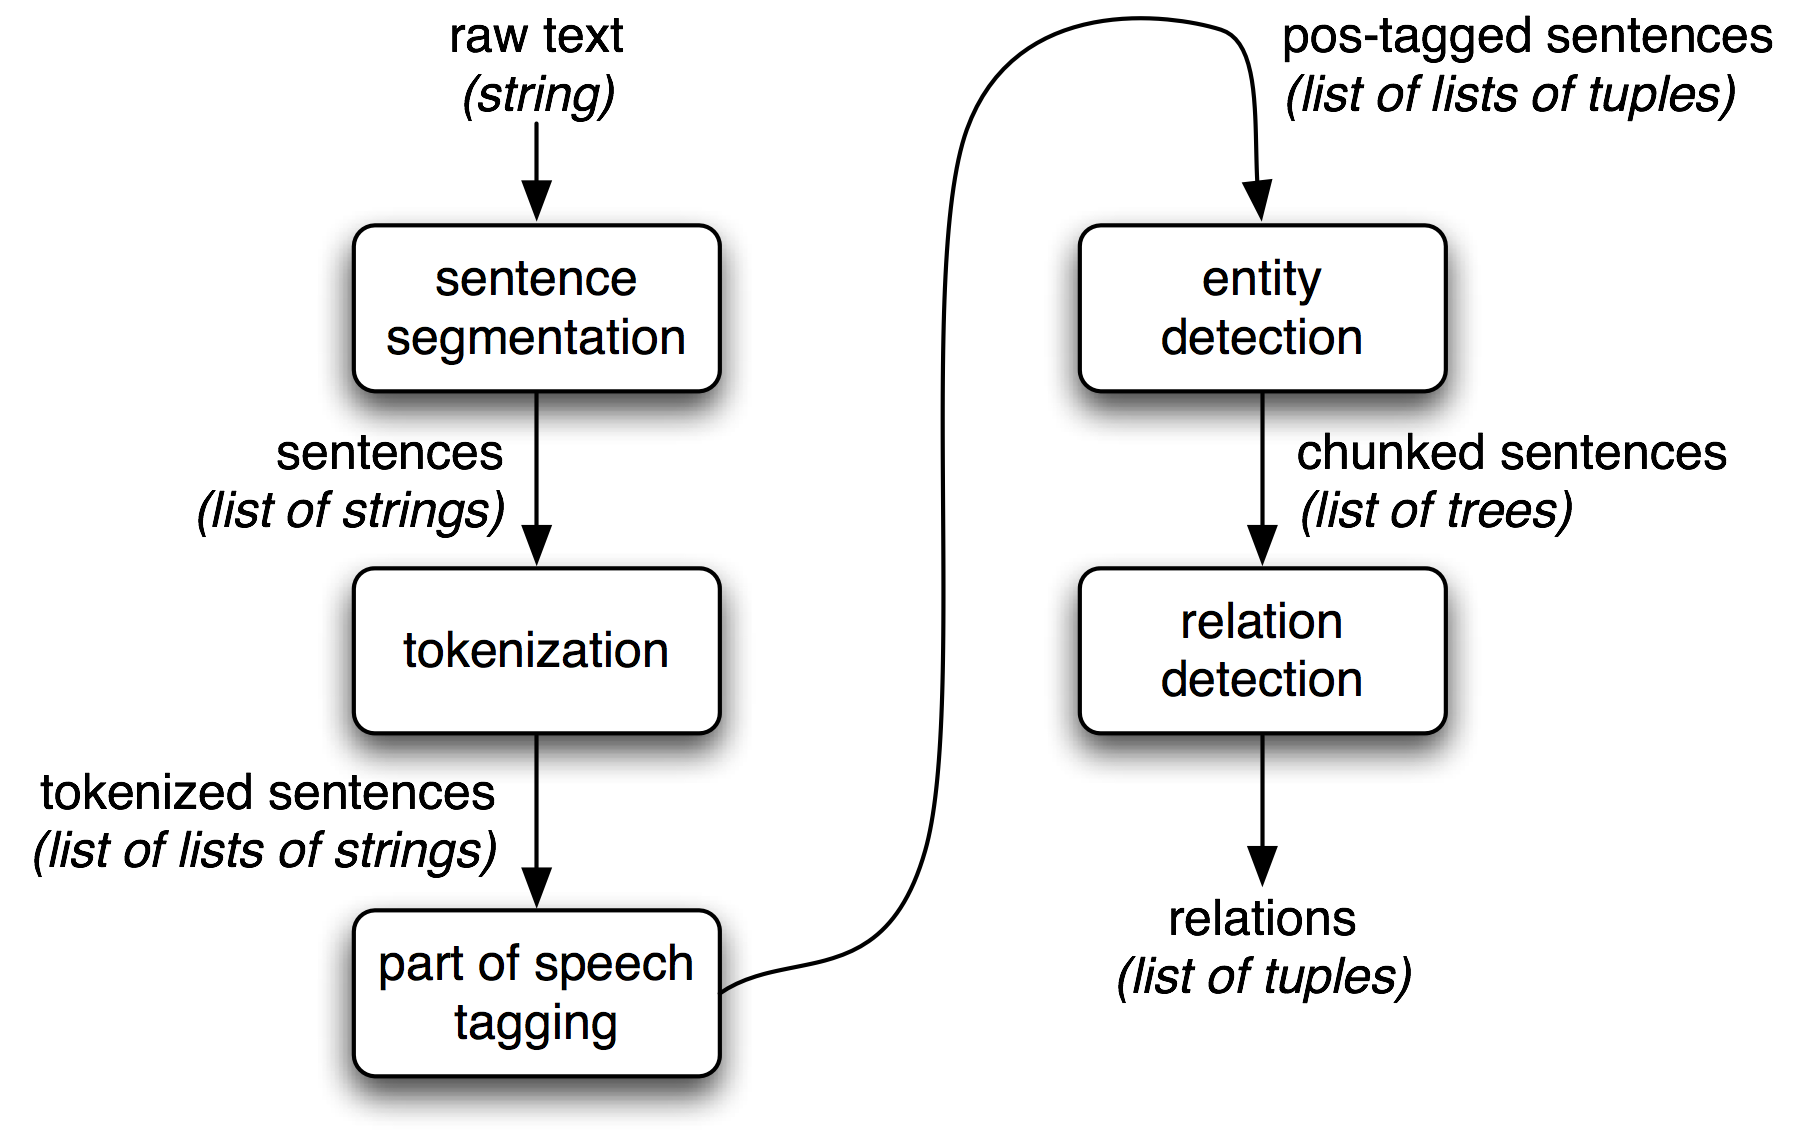
\includegraphics[scale=0.7]{images/pos.png}\label{tree}
\end{figure}
\section{ Named Entity Recognation and Classification   (NERC)}

The term "Named entity" has been coined in 1996 by  \citep{grishman1996design}.
Entity can be referred as a task, the entity is "named" when it is restricted to one or many rigid designators \citep{sharnagat2014named} such as persons, locations, product etc.

Based on the classification of Standard Generalizes Markup Language (SGML) a task can be divided into three subtasks:
\begin{enumerate}
\item ENAMEX: locations, products, organizations
\item NUMEX : percentage, quantity
\item TIMEX : time, date
\end{enumerate}
During a process of classification, Capitalization can be used in different ways such as the beginning of the proper noun, the abbreviation, the post of high level profile people etc.

Considering the English language text, if we are given a  particular token it is not by chance  to  determine whether it is a name or not. Some of the approaches to indicate a name are to  use capitalization  detection of sentence boundaries and dictionaries \citep{baluja2000applying}.

To handle this ambiguity, some systems use the special purpose-regular expression grammar, exception rule method, and so on.  David Palmer and Marti Hearst in  \citep{palmer1994adaptive} worked on punctuation marks and capitalization of words. They developed an efficient system with high accuracy in automatic sentences boundaries labelling   by using the feed forwarding neural-networks where the input was the Part-of-speech (POS) probabilities of all tokens which are surrounding the punctuation. Their output was found as the label of tokens.  David Palmer and Marti Hearst 's work was able to find correctly $98.5\%$ for punctuation of  sentence-boundaries. A proposed  new approach was how to represent the context of punctuation marks without ambiguities.

%\section{Mathematics  behind extraction}
%\Jnote{by me: do introduction to this part}
For extracting entities in a report there are different models which can be used like Hidden Markov model, Supporting Vector Machine (SVM), etc.

\section{Hidden Markov Model (HMM)}
It is a statistical Markov model which trains randomly systems and assumes that future states depend on current trained states.
HMM is specifically used for extraction of patterns in texts and speeches.
This model is based on Bayesian probability inference which has been initiated in 18th century. HMM is the earliest applied model for Natural Entities Recognition for English language.The way to perform these tasks is to find the most likely sequence of tagged names TN given a sequence of words "SW".

\begin{align}
P(TN|SW) & = \frac{P(SW|TN)P(TN)}{P(SW)}\label{eq2.0.1}
\end{align}
The equation  \eqref{eq2.0.1} is conditional probability, $P(TN|SW)$ can be  called posterior and it is  the probability of an event   tagged names occurring given sequence of word has observed.
%\Jnote{Formula and explanation above are inconsistent.}
$P(SW|TN)$ is also called likelihood e.i.  it is the probability of observing the sequence of words SW when the given hypothesis tagged name  TN is true. On the other handP(TN) doesn’t depend on the evidences, P(TN) is called prior e.i.  that it is true even if there is no given evidence at all. 
We can be ignore P(SW) and the remaining objective is to maximise the probability of getting the sequence of tagged names when sequence of words is given.
\begin{align}
Max\left[P(TN|SW)\right] \label{eq2.0.2}
\end{align} Due to assumption that the probabilities of tags are independent from each other,  from maximization equation \eqref{eq2.0.2},  we can  can get 
\begin{align}
P(TN){\approx} \prod_{i=1}^{n} P({TN}_{i}|{TN}_{i-1})\label{2.0.3}
\end{align}
Where ${TN}_{i}$ is a tag in the sequence of names (TN), for the likelihood probability can be estimated as :
\begin{align}
P(SW|TN){\approx}\prod_{i=1}^{n} P({SW}_{i}|{TN}_{i})\label{2.0.4}
\end{align}
The above estimations was for a small sequence where ${TN}_{i}$ is a tag in the sequence of names (TN) and ${SW}_{i}$ is a tag at index i in a sequence words (SW). For the large training corpus, the needed step is estimate based on the number of times the tag occurs and the position of the tag in a given corpus.
\begin{align}
P(T_{i}|T_{i-1}) = \frac{K(T_{i-1},T_{i})}{K(T_{i-1})}\label{2.0.5}
\end{align}
Based on the training corpus, $K(T_{i-1},T_{i})$ is referred as a how many times the tag $T_{i}$ occurs after the tag $T_{i-1}$. In the corpus, $K(T_{i-1})$ is considered as the number of occurrences for the tag $T_{i-1}$.

Therefore the estimation can be performed as follow:
\begin{align}
P(C_{i}|T_{i}) =  \frac{K(T_{i},C_{i})}{K(T_{i})} \label{2.0.6}
\end{align}
From the equation \eqref{2.0.6}, the term $K(T_{i},C_{i})$  is referred as the sum of the times that a word "$C_{i}$" has a tag $T_{i}$ in the training corpus.
The process of computing the posterior using the above steps is called Markov model.

It is one of the most powerful statistical and machine learning (ML) techniques in modelling and high qualified in entities extraction. When the researcher is willing to train new data, HMM is very robust and efficient in computations.
%\section{2.1.1.2. Disadvantages of Hidden Markov Model}
One of the limitations of HMM is that the researcher must have the notion of model topology and statistical techniques on how to deal with large amount of training data.
\section{Supporting Vector Machine (SVM) based model}
This model has an aim of classifying the named entities by separating the documents into two categories.  The document must belong to one category, either positive or negative.  SVM can classify linear data as well as non linear with a purpose of maximizing the margin between negative and positive documents.The plane which separate those two categories is called "hyperplane".

The main idea behind SVM modelling is to work with features and find the hyperplane. The hyperplane must separate all given samples regardless the dimensions.

\subsection{Linear Supporting Vector Machine }
For linear sample data, it is simple to plot the hyperplane to handle the separation.  Data are spread separately between positive documents and negative documents. The way data are represented SVM decided  whether to use linear modelling or not. IFRC reports are considered as multi dimensional documents.
\newpage                                                                                                                                                                                                                                          
\begin{figure}
\caption{Two dimensional SVM \citep{moreira2013finding}}
 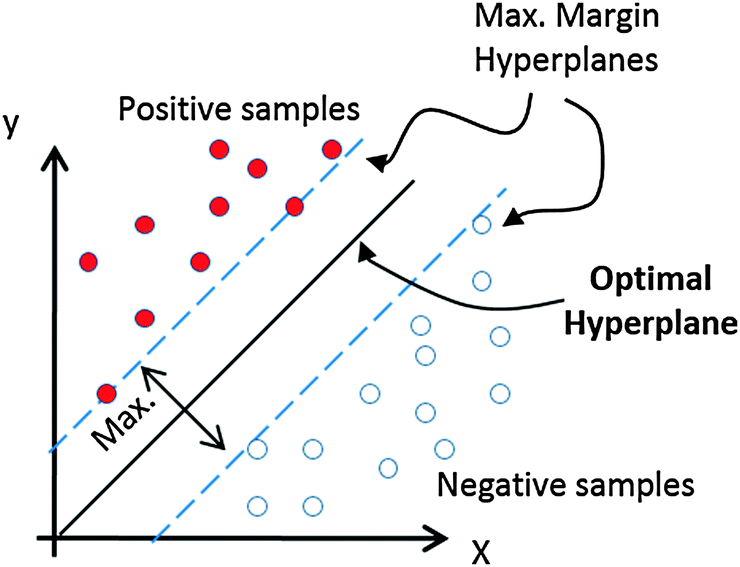
\includegraphics[scale=.4]    	          {images/linear.png} \label{linear}
\end{figure}  

In Figure \ref{linear}, blue circles represent negative documents and red circles represent positive documents.
The aim of SVM is to maximize the margin between negative documents and positive documents. Hyperplane is perpendicular. Optimal hyperplane separate perfectly two categories for two dimensional data.
 
Multidimensional documents whith separated classes are represented in Figure \ref{MDSVM}
\begin{figure}[hbtp]
\caption{Multi dimensional SVM}
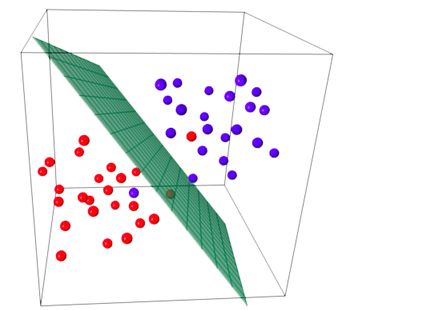
\includegraphics[scale=.6]{images/multi.png}\label{MDSVM}
\end{figure}

Documents classes are clearly separated as shown in Figure \ref{MDSVM}. we have positive samples on right hand side and negative samples on left hand side. for multidimensional representation, hyperplane is a plane instead of a line. When documents are mixed, hyperplane can't not be neither a straight plane nor a straight line. samples documents are classified as non linear documents.
\newpage
\subsection{Non Linear data} 
Sometimes the representation of data is quite mixed way so that you cant plot hyperplane easily. When the hyperplane can not be plotted as a straight line,  SVM looks for a way to linearise them by using a function. $ \phi$ maps data to the higher dimensional space. Straightforwardly, the classification became linear. Figure \ref{SVMNL} shows the way a function $ \phi$ linearised the data.



\begin{figure}[hbtp]
\caption{Nonlinear SVM classification \citep{moreira2013finding}}
\centering
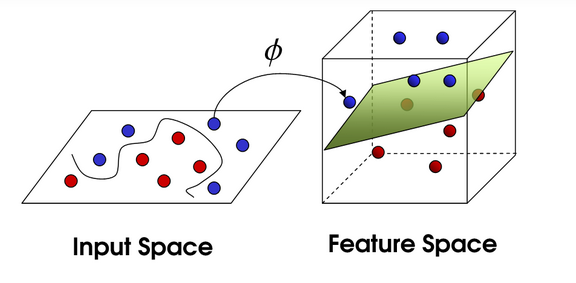
\includegraphics[scale=.7]{images/SVMNL.png}\label{SVMNL}
\end{figure}

However, SVM has some disadvantages in classification. Some particular documents can not be  easily performed without destroying the constructed weights  but this can not happen for  hand-written rule model. Machine learning uses decision tree procedure rather than  SVM.
%In addition the decision tree has a detailed boolean-like  model which is  mostly used. 

\section{Extraction before Machine learning}
Before the evolution of machine learning algorithms, NLP was using some  techniques to extract needed information in documents like:

\textit{Hand-written rule}

It is one of the standard approaches of NER and IE, it has been used for extracting the patterns from automated pages such as amazon, NLP was using hand- written regular expressions for unstructured humman-written text by delivering  part-of-speech (POS), syntactic parsing and categories of semantic words.

\textit{Rule /pattern based extraction}

Many IE systems uses rule/pattern to extract words and also phrases by looking to the context of those words or based on the their surroundings.\citep{califf2003bottom}. Some system decided if the procedure of extracting the words should rely on the meaning of each word independently or on the context of their surroundings in a phrase.
The limitation of this method is that some words do not have a closer mining to their surroundings that is why Patwardhan Siddharth with  Ellen Rilo  in workshop called "ACL 2006" presented another approach which  was  generating an automated IE system to learn patterns from a large fixed data set  within a specific domain \citep{patwardhan2007effective} 

Our research deals with reports generated through a template, compared to the work of  \citep{patwardhan2007effective} templates usages is a limitation.

\section{Text classification and Naive Bayes}


It is one of the most important algorithm in text classification by using base rule and bag of words to classify the entities \citep{manning2012information}.The user instead of going through the report and start posing many queries, text classification algorithm transient the need information.
Its aims is to build a function $\theta$ which takes the bag of words and returns the class of sentiment $C$ either positive or negative.
 
{\centering{$\theta$}

\centering{$\Updownarrow$}   

\begin{figure}[hbtp]
%\caption{a part of a sample reeport}
\centering
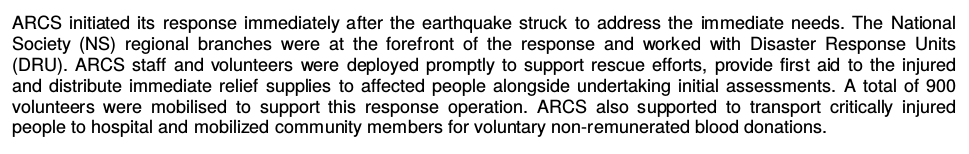
\includegraphics[scale=0.5]{images/report.png}\label{report}
\end{figure}

{\centering{$\Updownarrow$}}

{\centering{C}}

}
The classes of documents are mostly used in sentiment analysis. For example for social media where readers can say if they like the article or not.

For class analysis, we look for every word. but there exist another way to consider some subset of word and ignore other words.
The procedure is to look for all words and retrieve those which form the subsets.  Bag of words are formed after throwing away  all words except the subsets.The use of the function $\theta$  is for  attributing  to each item of the bag of words a sentiment. The function $\theta$  assigns every word a class based on high probability.

%\Jnote{I did not understand what this algorithm is for and how it works. I don't see how the picture is relevant to the algorithm.Please provide the source for the picture.}

\section{Machine learning for Named Entities\label{Chapter2}}
The natural language processing is not enough to handle the sophistication and ubiquity of textual data. Deep learning using machine learning techniques has been introduced to solve this problems. The advantages of machine learning for Named Entities:
\begin{itemize}
\item Manual extraction of entities is too expensive.
\item Fast processes of extraction.
\item Extraction is done by learning algorithms and natural language tools.
\item No limitation of languages due to polyglot package .
\end{itemize}





